

\documentclass[journal]{IEEEtran}

\usepackage{graphicx}
\begin{document}


\title{Development of a Human Movement Codec}


\author{David~Chiasson}

\maketitle

\begin{abstract}
Real-time kinematic data is central to many emerging technology applications, yet to date few techniques have been proposed to process and represent with this relatively new information modality in an efficient manner. This paper explores techniques for the compression of human kinematic data. Techniques from traditional multimedia networks are compared with several novel approaches. Simple, computationally cheap techniques are shown to losslessly compress kinematic data by over a factor of ten compared with traditional representations. Furthermore, these simple techniques are shown to be superior to more complex approaches.
All techniques discussed in this study are implemented and released as open source code which can be quickly integrated into a variety of computational platforms. 
\end{abstract}

\begin{IEEEkeywords}
kinematic data, human movement, compression, codec
\end{IEEEkeywords}



\section{Introduction}

\IEEEPARstart{M}{any} emerging technology applications rely on on real-time kinematic data as a crucial component. These include virtual reality, autonomous driving, internet of things, physical therapy, wearable electronics, and human performance among others. These applications have been enabled by the recent explosion of cheap inertial based sensors (IMUs) along with mobile computation power to process this data at high sampling frequency. Kinematic data represents a nascent field of multimedia data which is starkly under-developed compared to the existing maturity of text, audio, and visual type data processing techniques. In order to enable the modern applications listed above, efficient and standard techniques for representing and processing kinematic data are needed.

This study explores a range of both traditional and novel compression techniques applied to human kinematic data gathered by 6-axis IMUs. The best performing techniques are identified and discussed. Only lossless compression techniques are considered. The reason for this is that lossy compression inherently involves a value judgment about what information is useful and what information is irrelevant. In the absence of a specific application, no justification can be made for discarding any portion of information.

This study focuses on highly practical approaches which can be used in modern applications. To demonstrate this, all compression techniques have been implemented and released as open-source C code using fixed point computations. The hope of the authors is that this code can be a starting point for academic or industry developers implementing some kinematic data application on any type of computational platform.

All compression algorithms can be divided into two phases, modeling and coding[TO CITE] as shown in figure \ref{fig:general_compressor}. The model incorporates our knowledge about the signal to be compressed. It computes a probability mass function (PMF) which is an estimated likelihood of all possible input symbols. A dynamic model is one which changes its PMF estimate after new input symbols are received. The coder then reads the uncompressed data and uses the PMF to choose a unique code for each input symbol. Short codes are chosen for likely symbols and long codes are chosen for unlikely symbols such that the total length of the compressed data is minimized. The decompressor uses an identical model to provide the same PMF to the decoder which is used to revert each code back into the original symbol. If the model is dynamic, this output is used to update the model for future predictions. Coding is a solved problem and will thus not be discussed in this work.[TO CITE] Modeling on the other hand has been proven unsolvable and must be revisited for each new class of signal.(due to the pidgeon hole principal?)[TO CITE]. To the author's knowledge, no previous work has directly addressed the modeling problem for kinematic data signals. This provides the motivation for the current work. Modeling has been shown to be equivalent to the artificial intelligence problem [TO CITE].

\begin{figure}
  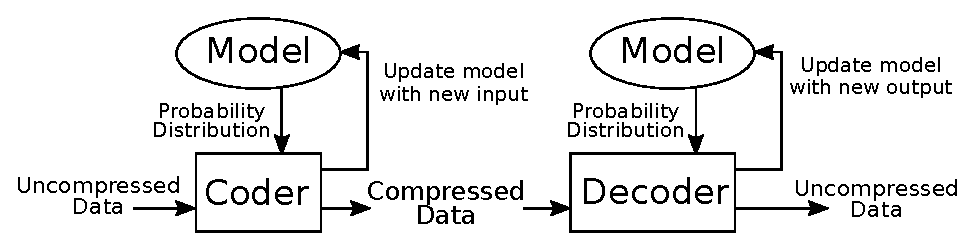
\includegraphics[width=\linewidth]{general_compressor.eps}
  \caption{General compressor and decompressor}
  \label{fig:general_compressor}
\end{figure}

We hypothesize that compression ratios will be comparable to those achieved in lossless audio compression. We also hypothesize that the best performing codec will utilize some cross axis correlation and be informed by physics based models.

\section{Method}
In order to meaningfully and repeatable demonstrate the performance of a compression algorithm, a public kinetic signal corpus must be selected. For this study, the Human Gait Database (HuGaDB) is used. HuGaDb is a public dataset of six-axis IMU signals collected from six different body segments of 18 healthy subjects performing 12 different movement activities[TO Cite]. This database was selected because it allowed the comparison of compression techniques across body segment, subject, and activity in addition to sensor modality.

The data collected from three random subjects was designated as training data, and only data from the remaining 15 subjects was used in our results. The training data was used to train the lasso regression of our cross-stream FIR filter discussed later.

\subsection{Reference Encodings}
As it has been proven impossible to claim maximum compression [TO CITE] it is necessary to select a reference when evaluating the performance of a compression algorithm. In this study, the baseline encoding (exhibiting a compression ratio of one) is comma separated value (CSV), a simple text based format which is the de-facto standard for storing sensor information. To give further context to performance, established algorithms from both text and audio compression are applied to the kinematic data. In total, the following five reference encodings are used to give context to compression ratios:

\begin{itemize}
  \item \textbf{CSV} Standard text based format
  \item \textbf{Binary} The optimal fixed size format. In our corpus, every sample is two bytes.
  \item \textbf{Binary Rice Encoded} Binary files with Rice-Golomb encoding[TO CITE] applied. This would be the optimal compression if each sample were an IID geometrically distributed random variable with mean zero.
  \item \textbf{ZIP compression of CSV} ZIP is a general purpose compressed file format used in most computer systems. [TO CITE] (include options)
  \item \textbf{FLAC compression of binary} FLAC is a popular, open-source lossless audio codec (include options)[TO CITE]
\end{itemize}
\subsection{Tested Encodings}



fixed point requirement

lossless, causal, node independent
\begin{itemize}
  \item \textbf{Delta encoding}
  \item \textbf{Linear extrapolation}
  \item \textbf{\boldmath$2^{nd}$ to \boldmath$5^{th}$ order polynomial prediction}
  \item \textbf{Spline extrapolation}
  \item \textbf{Linearized rotating gravity}
  \item \textbf{Cross stream FIR filter}
\end{itemize}

\subsection{Implementation}
flow chart

\begin{figure}
  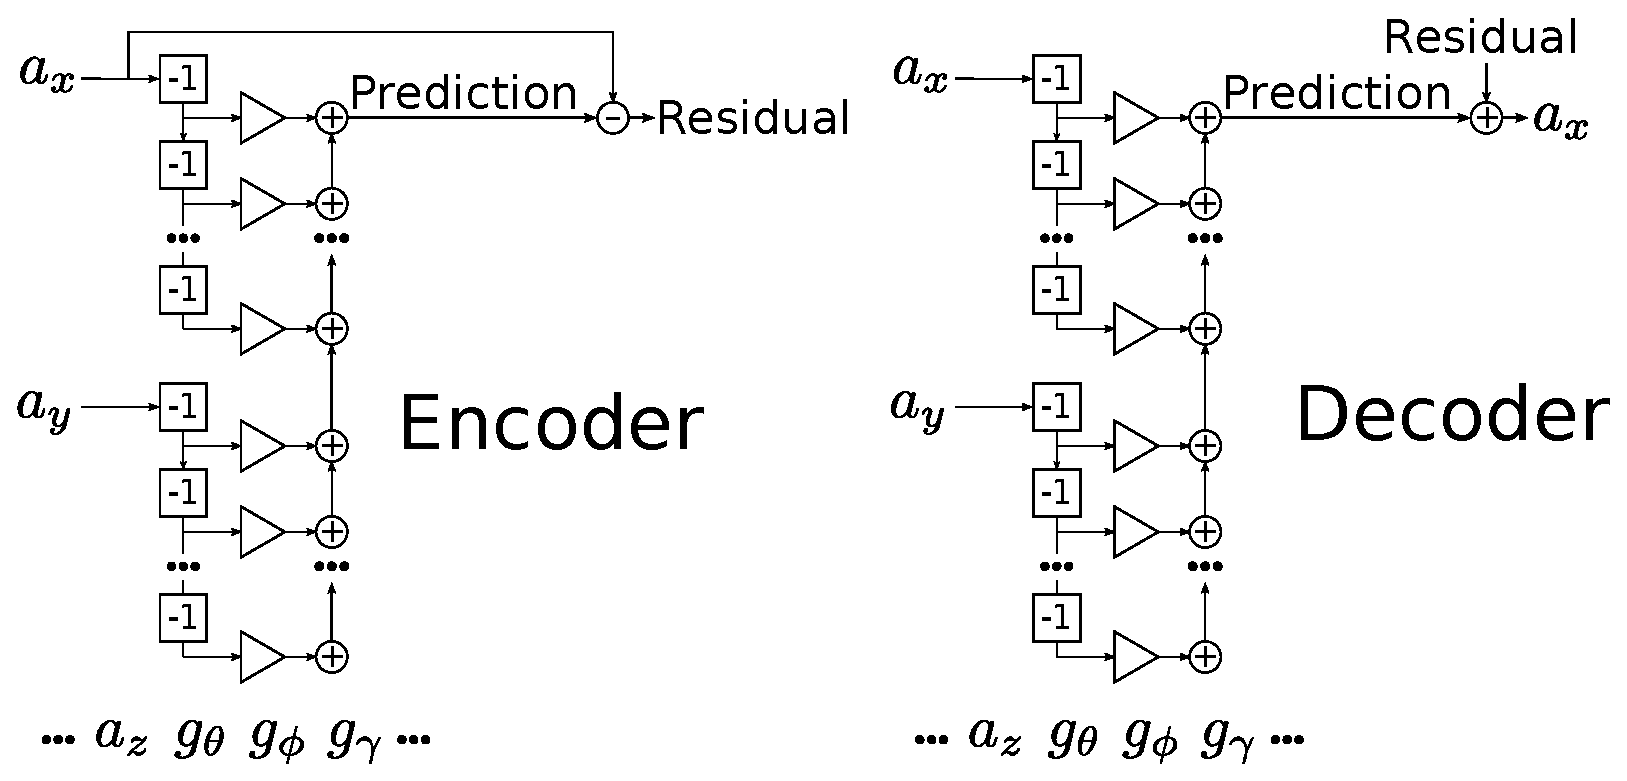
\includegraphics[width=\linewidth]{flow_diagram.eps}
  \caption{Flow diagram of encoder and decoder.}
  \label{fig:flow_diagram}
\end{figure}

Figure \ref{fig:flow_diagram} shows a boat.


released open-source link
\section{Results}
Single bar graph of best compression

Tables of detailed results k, order: total, accel/gryo, activity, segment, subject 

Discussion of cross stream FIR coefficents, pole zero plots
\section{Discussion}
Significant easy gains important for pracitce

Compression ratio variance by movement and placement

Was poor performance of complex algorithms due to precision issues?

Surprising performance of difference encoding

Lack of correlation between accelerometer and gyroscope

Compression rate compared to audio

Future work: lossy, multiple hardware/sampling rates, other body parts

improvements: dynamic K, blocking for error recovery

\section{Conclusion}
Kabam! Splat!


% use section* for acknowledgment
\section*{Acknowledgment}

The authors would like to thank your mom.

\begin{thebibliography}{1}

\bibitem{IEEEhowto:kopka}
H.~Kopka and P.~W. Daly, \emph{A Guide to \LaTeX}, 3rd~ed.\hskip 1em plus
  0.5em minus 0.4em\relax Harlow, England: Addison-Wesley, 1999.

\end{thebibliography}

\end{document}